\documentclass[12pt, a4paper]{article}

% ==========================================
% 1. KHAI BÁO GÓI THƯ VIỆN (PACKAGES)
% ==========================================
% Bảng mã & Font chữ
\usepackage[utf8]{inputenc}
\usepackage[T5]{fontenc}

% Toán học
\usepackage{amsmath, amssymb}

% Căn lề & Bố cục trang
\usepackage[top=2.2cm, bottom=1.5cm, left=1cm, right=1cm, headheight=15pt]{geometry}
\usepackage{fancyhdr}
\usepackage{needspace}
\usepackage{tkz-tab}
\usepackage{float}

% Đồ họa & Màu sắc
\usepackage{xcolor}
\usepackage{graphicx} 
\usepackage{tikz}
\usetikzlibrary{calc, shapes.geometric, positioning}


% Bảng biểu & Danh sách
\usepackage{colortbl}
\usepackage{array}
\usepackage{makecell}
\usepackage{multirow}
\usepackage{tasks}

% Biểu tượng
\usepackage{fontawesome5}

% ==========================================
% 2. THIẾT LẬP MÀU SẮC CHỦ ĐẠO
% ==========================================
\definecolor{goldyellow}{RGB}{255, 179, 0}
\definecolor{amberorange}{RGB}{230, 115, 0}
\definecolor{lightamber}{RGB}{255, 248, 225}
\definecolor{deepblue}{RGB}{25, 42, 86}
\definecolor{accentred}{RGB}{232, 65, 24}
\definecolor{softgray}{RGB}{220, 220, 222} 
\definecolor{fbblue}{RGB}{15, 80, 200}


% ==========================================
% 3. CẤU HÌNH HEADER & FOOTER
% ==========================================
\pagestyle{fancy}
\fancyhf{}
\renewcommand{\headrulewidth}{0pt}

% Khai báo biến lưu trữ nội dung góc phải của Header
\newcommand{\HeaderRightText}{}

% --- Header ---
\fancyhead[C]{
    \begin{tikzpicture}[remember picture, overlay]
        
        % Dải màu trang trí góc trên
        \path[fill=deepblue] (current page.north west) -- (current page.north east) 
            -- ($(current page.north east) + (0, -1.6cm)$) 
            .. controls ($(current page.north) + (3, -2.0cm)$) and ($(current page.north) + (-3, -0.4cm)$) .. 
            ($(current page.north west) + (0, -1.0cm)$) -- cycle;
            
        \path[fill=goldyellow] (current page.north west) -- (current page.north east) 
            -- ($(current page.north east) + (0, -1.0cm)$) 
            .. controls ($(current page.north) + (4, -1.0cm)$) and ($(current page.north) + (-2, -2.2cm)$) .. 
            ($(current page.north west) + (0, -1.6cm)$) -- cycle;
            
        \path[fill=amberorange] (current page.north west) -- ($(current page.north west) + (6.5cm, 0)$) 
            .. controls ($(current page.north west) + (4.5cm, -1.2cm)$) and ($(current page.north west) + (2cm, -2.0cm)$) .. 
            ($(current page.north west) + (0, -2.0cm)$) -- cycle;
            
        % Logo góc trái Header
        \node[anchor=west, inner sep=0pt] 
            at ($(current page.north west) + (0cm, -0.8cm)$) {
\includegraphics[height=2.0cm]{../../../image/logo-header.png}};
            
        % Text góc phải Header (Tự động lấy từ đối số thứ 3 của \titlebox)
        \node[anchor=east, text=white, font=\small\bfseries\sffamily] 
            at ($(current page.north east) + (-0.8cm, -0.5cm)$) {\HeaderRightText};
    \end{tikzpicture}
}

% --- Footer ---
\fancyfoot[C]{
    \begin{tikzpicture}[remember picture, overlay]
        % Đường kẻ ngang
        \draw[amberorange, line width=1.5pt] 
            ($(current page.south west) + (0cm, 0.4cm)$) -- ($(current page.south east) + (0cm, 0.4cm)$);

        % Dải cong góc phải
        \path[fill=goldyellow] (current page.south east) -- ($(current page.south east) + (-5cm, 0)$) 
            .. controls ($(current page.south east) + (-3cm, 0.8cm)$) and ($(current page.south east) + (-1.5cm, 1.2cm)$) .. 
            ($(current page.south east) + (0, 1.2cm)$) -- cycle;

        % Mạng xã hội
        \node[anchor=west, inner sep=0pt] at ($(current page.south west) + (1cm, 0.8cm)$) {
            \small\sffamily
            \textcolor{fbblue}{\faFacebook\hskip 4pt Toán Anh Huy MATH-STER}
            \hskip 18pt
            \textcolor{black}{\faTiktok\hskip 4pt huymathster}
        };

        % Số trang
        \node[circle, fill=white, draw=amberorange, line width=1.5pt, text=deepblue, font=\large\bfseries\sffamily, inner sep=4pt, minimum size=0.8cm] 
            at ($(current page.south east) + (-1.2cm, 0.6cm)$) {\thepage};
    \end{tikzpicture}
}

% ==========================================
% 4. ĐỊNH NGHĨA MACRO: KHUNG TIÊU ĐỀ
% ==========================================
\newcommand{\titlebox}[3]{
    % Gán nội dung đối số #3 vào biến HeaderRightText
    \gdef\HeaderRightText{#3}
    
    \begin{center}
    \vspace*{-0.5cm}
    \begin{tikzpicture}
        % Khung vô hình (Phantom Box) định chuẩn kích thước
        \node[text width=16cm, inner xsep=0pt, inner ysep=16pt, opacity=0] (MainBox) {
            \begin{minipage}[c]{4.2cm}
                \centering\vspace{0.1cm}
                \rule{2.2cm}{2.2cm} 
                \vspace{0.1cm}
            \end{minipage}%
            \begin{minipage}[c]{11.5cm}
                \centering\vspace{0.15cm}
                {\huge\bfseries\sffamily #2 \par}
                \vspace{0.15cm} 
            \end{minipage}
        };
        
        % Đổ bóng & Nền
        \fill[goldyellow, rounded corners=8pt] ([xshift=5pt, yshift=-5pt]MainBox.south west) rectangle ([xshift=5pt, yshift=-5pt]MainBox.north east);
        \fill[white, rounded corners=8pt] (MainBox.south west) rectangle (MainBox.north east);
        
        % Lưới ô ly & Nền Logo
        \begin{scope}
            \clip[rounded corners=8pt] (MainBox.south west) rectangle (MainBox.north east);
            \draw[step=0.4cm, softgray!50, line width=0.6pt] (MainBox.south west) grid (MainBox.north east);
            \fill[lightamber!60] (MainBox.south west) rectangle ([xshift=4.2cm]MainBox.north west);
        \end{scope}

        % Viền ngoài
        \draw[deepblue, line width=1.5pt, rounded corners=8pt] (MainBox.south west) rectangle (MainBox.north east);

        % Nội dung Text (Lớp trên cùng)
        \node[text width=16cm, inner xsep=0pt, inner ysep=16pt] at (MainBox.center) {
            \begin{minipage}[c]{4.2cm}
                \centering
                % --- ĐIỀU CHỈNH TỌA ĐỘ LOGO Ở ĐÂY ---
                \hspace*{-0.5cm}\raisebox{-0.2cm}{
\includegraphics[width=5.5cm]{../../../image/logo.png}}
            \end{minipage}%
            \begin{minipage}[c]{11.5cm}
                \centering\vspace{0.15cm}
                {\huge\bfseries\sffamily\color{deepblue} #2 \par}
                \vspace{0.15cm} 
            \end{minipage}
        };
        
        % Trang trí phụ kiện
        \draw[deepblue, line width=1.5pt, dashed] ([xshift=4.2cm]MainBox.north west) -- ([xshift=4.2cm]MainBox.south west);
        \node[regular polygon, regular polygon sides=4, rotate=45, fill=white, draw=accentred, line width=1.2pt, inner sep=2.5pt] at ([xshift=4.2cm]MainBox.west) {};
        \node[anchor=west, fill=amberorange, text=white, font=\large\bfseries\sffamily, rounded corners=4pt, draw=deepblue, line width=1.5pt, inner xsep=12pt, inner ysep=6pt] at ([xshift=1.5cm]MainBox.north west) {#1};
        \fill[accentred] ([xshift=-1.8cm, yshift=-0.4cm]MainBox.north east) circle (3pt);
        \fill[amberorange] ([xshift=-1.4cm, yshift=-0.4cm]MainBox.north east) circle (3pt);
        \fill[goldyellow] ([xshift=-1.0cm, yshift=-0.4cm]MainBox.north east) circle (3pt);
    \end{tikzpicture}
    \vspace*{0cm}
    \end{center}
}

% ==========================================
% 5. ĐỊNH NGHĨA MACRO: CẤU TRÚC CÂU HỎI (ÉP SÁT NHAU)
% ==========================================
\newcommand{\questioncore}[2]{
    % Xóa khoảng cách phía trên, ép sát câu trước
    \noindent \textbf{\textcolor{deepblue}{Câu #1.} \textcolor{accentred}{[STER]}} #2
    \par\nopagebreak
}

% Cấu hình hiển thị đáp án trắc nghiệm
\settasks{
    label=\textbf{\textcolor{amberorange}{\Alph*.}}, 
    label-width=15pt,     
    item-indent=25pt,     
    label-offset=6pt,    
    column-sep=20pt,     
    after-item-skip=2pt  % Đã giảm tối đa khoảng cách giữa các dòng đáp án A B C D
}

% Hàm vẽ dòng kẻ nháp
\newcommand{\drawdashlines}[1]{
    \ifnum#1>0
        \nopagebreak\vspace{0.1cm}\noindent 
        \begin{tikzpicture}
            \foreach \i in {1,...,#1} {
                \draw[softgray, line width=0.2pt] (0,-{\i*0.75}) -- (\textwidth-4pt,-{\i*0.75});
            }
        \end{tikzpicture}
        \par
    \fi
    % Đã xóa hoàn toàn khoảng cách thừa ở nhánh else
}

% --- Dạng 1: Trắc nghiệm 4 đáp án ---
\newcommand{\questionLinesManual}[4]{
    \pgfmathsetmacro{\calculatedSpace}{1.5 + #1 * 0.65}
    \needspace{\calculatedSpace cm} 
    \questioncore{#2}{#3}
    #4
    \par\nopagebreak
    \drawdashlines{#1}
}

% --- Dạng 2: Trắc nghiệm Đúng/Sai ---
\newcommand{\questionTrueFalse}[4]{
    \pgfmathsetmacro{\calculatedSpace}{3.0 + #1 * 0.65} 
    \needspace{\calculatedSpace cm}
    \questioncore{#2}{#3}
    
    \nopagebreak
    \begin{center}
    \renewcommand{\arraystretch}{1.8} % Bóp nhỏ chiều cao của bảng Đ/S
    \begin{tabular}{|>{\centering\arraybackslash}m{0.8cm}|m{12cm}|>{\centering\arraybackslash}m{2cm}|>{\centering\arraybackslash}m{2cm}|}
        \hline
        \rowcolor{amberorange!20}
        & \multicolumn{1}{>{\centering\arraybackslash}m{12cm}|}{\textbf{\textcolor{deepblue}{Mệnh đề}}} & 
        \textbf{\textcolor{deepblue}{Đúng}} & 
        \textbf{\textcolor{deepblue}{Sai}} \\
        \hline
        #4
        \hline
    \end{tabular}
    \renewcommand{\arraystretch}{1}
    \end{center}
    
    \par\nopagebreak
    \drawdashlines{#1}
}

% ----- Dạng 3: Tự luận ngắn -----
\newcommand{\questionShortAnswer}[3]{
    \pgfmathsetmacro{\calculatedSpace}{1.5 + #1 * 0.8}
    \needspace{\calculatedSpace cm}
    
    {\linespread{1.1}\selectfont % Bóp nhỏ giãn dòng của câu tự luận
    \questioncore{#2}{#3}\par}
    
    \nopagebreak
    \begin{flushright}
        \begin{tikzpicture}
            \node[anchor=east, font=\small\bfseries\sffamily, text=deepblue] 
                at (-0.2, 0.4) {Đáp án:};
            \fill[goldyellow, rounded corners=3pt] (0.08, -0.08) rectangle (3.08, 0.72);
            \draw[draw=deepblue, fill=white, line width=1.2pt, rounded corners=3pt] 
                (0,0) rectangle (3.0, 0.8);
            \foreach \x in {0.75, 1.5, 2.25} {
                \draw[draw=deepblue, line width=0.6pt] (\x, 0) -- (\x, 0.8);
            }
        \end{tikzpicture}
    \end{flushright}
    
    \par\nopagebreak
    \drawdashlines{#1}
}

% ==========================================
% BẮT ĐẦU NỘI DUNG TÀI LIỆU
% ==========================================
\begin{document}

% Truyền 3 tham số: {Nhãn cam} {Chữ to chính giữa} {Chữ ở góc phải Header}
\titlebox{Chủ đề: Hàm số}{BTDD giá trị lớn nhất nhỏ nhất của quãng đường}{Hàm số: Min Max quảng đường}


% --- CÂU 1 ---
\questionTrueFalse{0}{1}{Một kho hàng được đặt tại vị trí A cách trục đường chính một khoảng \( AB = 8 \, km \). Trên trục đường đó có một trung tâm thương mại ở vị trí C cách B một khoảng \( BC = 20 \, km \) (tham khảo hình vẽ). Người giao hàng có thể đi xe máy từ vị trí A đến vị trí M trên trục đường chính với vận tốc 40 km/h và đi xe ô tô đến trung tâm thương mại C với vận tốc 60 km/h. Đặt \( BM = x \) với \( 0 < x < 20 \).
\begin{center}
    \begin{tikzpicture}[>=stealth, scale=1.3]

    % =================================================================
    % 1. ĐỊNH NGHĨA CÁC ĐIỂM CHÍNH TRÊN TRỤC HOÀNH VÀ ĐƯỜNG CAO
    % =================================================================
    % Trục nằm ngang kéo dài sang hai bên một chút
    \coordinate (StartLine) at (-0.5,0);
    \coordinate (EndLine) at (5.0,0);
    
    % Các điểm chính
    \coordinate (B) at (0.3,0);
    \coordinate (M) at (2.2,0);
    \coordinate (C) at (4.5,0);
    \coordinate (A) at (0.3,3.0);

    % =================================================================
    % 2. VẼ CÁC ĐƯỜNG THẲNG
    % =================================================================
    % Vẽ đường thẳng nằm ngang chính
    \draw[thick] (StartLine) -- (EndLine);

    % Vẽ đoạn thẳng đứng AB và đoạn thẳng nghiêng AM
    \draw[thick] (A) -- (B);
    \draw[thick] (A) -- (M);

    % =================================================================
    % 3. VẼ KÝ HIỆU GÓC VUÔNG VÀ ĐIỂM ĐẶC BIỆT
    % =================================================================
    % Ký hiệu góc vuông tại đỉnh B (nằm bên trái đoạn thẳng AB)
    \draw[thin] (B) ++(-0.18,0) -- ++(0,0.18) -- ++(0.18,0);

    % Điểm C được biểu diễn bằng một chấm tròn đen nhỏ
    \fill (C) circle (1.5pt);

    % =================================================================
    % 4. GÁN NHÃN CÁC ĐỈNH
    % =================================================================
    \node[left=3pt] at (A) {$A$};
    \node[below=3pt] at (B) {$B$};
    \node[below=3pt] at (M) {$M$};
    \node[below=3pt] at (C) {$C$};

\end{tikzpicture}
\end{center}
}{
    \textbf{a)} & Quãng đường đi từ A đến M là \( 64 + x^2 \, (km) \).
    & \textcolor{amberorange}{$\bigcirc$} & \textcolor{amberorange}{$\bigcirc$} \\ \hline
    
    \textbf{b)} & Thời gian đi từ A đến C là \( 40\sqrt{64 + x^2} + 60(20 - x) \) giờ.
    & \textcolor{amberorange}{$\bigcirc$} & \textcolor{amberorange}{$\bigcirc$} \\ \hline
    
    \textbf{c)} & Thời gian ngắn nhất đi từ A đến C là khoảng 29 phút.
    & \textcolor{amberorange}{$\bigcirc$} & \textcolor{amberorange}{$\bigcirc$} \\ \hline
    
    \textbf{d)} & Muộn nhất 7 giờ 1 phút người đó phải xuất phát từ vị trí A để có mặt tại C lúc 8h sáng.
    & \textcolor{amberorange}{$\bigcirc$} & \textcolor{amberorange}{$\bigcirc$} \\
}

% --- CÂU 2 ---
\questionTrueFalse{0}{2}{Trong một cuộc thi cắm trại, xóm Kim Nghĩa treo bóng nháy cho công trại, sao cho điểm đầu và điểm cuối của dây bóng nằm ở vị trí hai chân của cổng. Ban cán sự xóm muốn treo bóng sao cho nó tạo thành hình tam giác như hình vẽ, biết xà ngang chứa điểm C treo bóng cách mặt đất 15m và cổng trại AB rộng 50m. Đặt \( AM = x \) (\( 0 < x < 50 \)) (m).
\begin{center}
    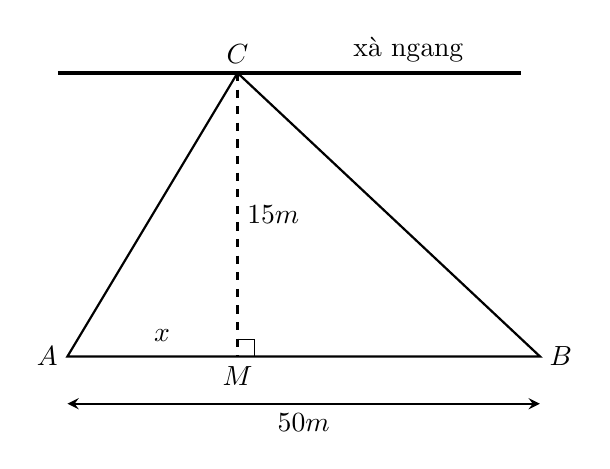
\begin{tikzpicture}[>=stealth, scale=1.2]

    % =================================================================
    % 1. ĐỊNH NGHĨA CÁC ĐIỂM CHÍNH TRONG TAM GIÁC
    % =================================================================
    \coordinate (A) at (0,0);
    \coordinate (B) at (5.0,0);
    \coordinate (M) at (1.8,0);
    \coordinate (C) at (1.8,3.0);

    % Tọa độ hai đầu của thanh xà ngang đi qua C
    \coordinate (XaTrai) at (-0.1,3.0);
    \coordinate (XaPhai) at (4.8,3.0);

    % =================================================================
    % 2. VẼ CÁC ĐƯỜNG LIỀN VÀ XÀ NGANG
    % =================================================================
    % Vẽ thanh xà ngang phía trên bằng nét siêu đậm
    \draw[ultra thick] (XaTrai) -- (XaPhai) node[above left, pos=0.9] {xà ngang};

    % Vẽ các cạnh của tam giác ABC
    \draw[thick] (A) -- (B) -- (C) -- cycle;

    % =================================================================
    % 3. VẼ ĐƯỜNG CAO CM (NẾT ĐỨT) VÀ GÓC VUÔNG
    % =================================================================
    \draw[dashed, thick] (C) -- (M);

    % Ký hiệu góc vuông tại M (nằm bên phải đường cao CM)
    \draw[thin] (M) ++(0,0.18) -- ++(0.18,0) -- ++(0,-0.18);

    % =================================================================
    % 4. GÁN NHÃN CÁC ĐỈNH VÀ THÔNG SỐ TRONG HÌNH
    % =================================================================
    \node[left] at (A) {$A$};
    \node[right] at (B) {$B$};
    \node[below] at (M) {$M$};
    \node[above] at (C) {$C$};

    % Điền giá trị độ dài x và 15m
    \node[above] at (1.0,0.05) {$x$};
    \node[right] at (1.8,1.5) {$15m$};

    % =================================================================
    % 5. VẼ MŨI TÊN KÍCH THƯỚC CHIỀU DÀI 50m PHÍA DƯỚI
    % =================================================================
    \draw[<->, thick] (0,-0.5) -- (5.0,-0.5);
    \node[below] at (2.5,-0.5) {$50m$};

\end{tikzpicture}
\end{center}
}{
    \textbf{a)} & Độ dài đoạn \( CB \) bằng \( \sqrt{15^2 + (50 - x)^2} \) (m).
    & \textcolor{amberorange}{$\bigcirc$} & \textcolor{amberorange}{$\bigcirc$} \\ \hline
    
    \textbf{b)} & Tổng đường dây bóng nối từ \( C \) đến \( A \) và từ \( C \) đến \( B \) là \( \sqrt{x^2 + 15} + \sqrt{(50 - x)^2 + 15} \) (m).
    & \textcolor{amberorange}{$\bigcirc$} & \textcolor{amberorange}{$\bigcirc$} \\ \hline
    
    \textbf{c)} & Khi \( x = 25 \) (m) thì tổng đường dây bóng cần nối là ngắn nhất.
    & \textcolor{amberorange}{$\bigcirc$} & \textcolor{amberorange}{$\bigcirc$} \\ \hline
    
    \textbf{d)} & Biết chi phí mỗi mét dây bóng có giá 15 000 đồng. Chi phí thấp nhất mà ban cán sự xóm cần trả là 874 643 đồng (kết quả làm tròn đến hàng đơn vị).
    & \textcolor{amberorange}{$\bigcirc$} & \textcolor{amberorange}{$\bigcirc$} \\
}


% --- CÂU 10 ---
\questionShortAnswer{0}{3}{Một người đưa thư đang ở điểm \( A \), cách điểm \( B \) một đoạn đường xuyên rừng dài \( 60 \, \text{km} \). Trong rừng, người này chỉ có thể di chuyển với vận tốc \( 25 \, \text{km/h} \), và người này cần đến \( B \) trong tối đa \( 2,25 \, \text{giờ} \). May mắn thay, có một con đường nhựa cách đoạn \( AB \) một khoảng \( 12 \, \text{km} \), chạy song song với nó. Trên đường nhựa, người này có thể di chuyển với vận tốc \( 45 \, \text{km/h} \). Biết rằng, nếu di chuyển trên đường nhựa thì người đó sẽ đi theo đường gấp khúc dạng hình thang cân \( ACDB \). Hỏi thời gian ngắn nhất để người đưa thư đi từ \( A \) đến \( B \) là bao nhiêu giờ (kết quả làm tròn đến hàng phần trăm)?

\begin{center}
\begin{tikzpicture}[>=stealth, scale=1.3]

    % =================================================================
    % 1. ĐỊNH NGHĨA TỌA ĐỘ CÁC ĐIỂM CHÍNH
    % =================================================================
    \coordinate (A) at (0,0);
    \coordinate (B) at (6.0,0);
    \coordinate (C) at (1.2,2.5);
    \coordinate (D) at (4.8,2.5);
    
    % Các đỉnh phụ để vẽ đường nét đứt thể hiện chiều cao hình thang
    \coordinate (TopA) at (0,2.5);
    \coordinate (TopB) at (6.0,2.5);
    
    % Giới hạn trục nằm ngang phía dưới
    \coordinate (LineStart) at (-0.7,0);
    \coordinate (LineEnd) at (6.7,0);

    % =================================================================
    % 2. VẼ CÁC ĐƯỜNG THẲNG LIỀN NÉT VÀ NÉT ĐỨT
    % =================================================================
    % Đường nền nằm ngang phía dưới đi qua A và B
    \draw[thick] (LineStart) -- (LineEnd);

    % Đường nhựa nằm ngang phía trên (bao gồm cả các đoạn kéo dài sang hai bên)
    \draw[thick] (TopA) -- (TopB);

    % Hai đường xiên AC và BD
    \draw[thick] (A) -- (C);
    \draw[thick] (B) -- (D);

    % Hai đoạn thẳng đứng thể hiện chiều cao vuông góc (nét đứt)
    \draw[dashed, thick] (A) -- (TopA);
    \draw[dashed, thick] (B) -- (TopB);

    % =================================================================
    % 3. VẼ CÁC ĐIỂM NÚT (CHẤM TRÒN ĐEN)
    % =================================================================
    \fill (A) circle (1.8pt);
    \fill (B) circle (1.8pt);
    \fill (C) circle (1.8pt);
    \fill (D) circle (1.8pt);

    % =================================================================
    % 4. GÁN NHÃN ĐỈNH VÀ ĐIỀN CHÚ THÍCH CHỮ
    % =================================================================
    % Nhãn các điểm hình học
    \node[below left] at (A) {$A$};
    \node[below right] at (B) {$B$};
    \node[above left] at (C) {$C$};
    \node[above right] at (D) {$D$};

    % Thông số khoảng cách/chiều cao 12km
    \node[left=3pt] at (0,1.25) {$12km$};

    % Các nhãn văn bản chú thích địa hình
    \node[above] at (3.0, 2.5) {Đường nhựa};
    \node at (3.0, 1.2) {Rừng};
    \node[below] at (3.0, -0.1) {Rừng};

\end{tikzpicture}
\end{center}}


% --- CÂU 13 ---
\questionShortAnswer{0}{4}{Hai con tàu A và B đang ở cùng một vĩ tuyến và cách nhau 6 hải lí. Cả hai tàu đồng thời cùng khởi hành. Tàu A chạy về hướng Nam với vận tốc 5 hải lí/giờ, còn tàu B chạy về vị trí hiện tại của tàu A với vận tốc 6 hải lí/giờ. Hỏi sau bao nhiêu giờ thì khoảng cách giữa hai tàu là ngắn nhất (kết quả làm tròn đến hàng phần trăm)?
\begin{center}
    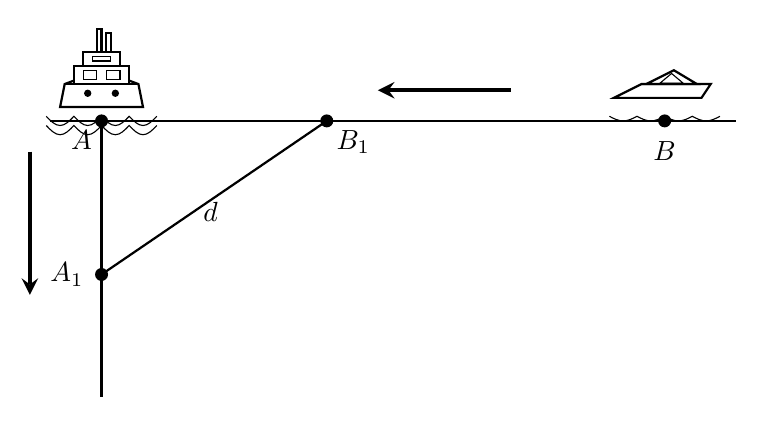
\begin{tikzpicture}[>=stealth, scale=1.3]

    % =================================================================
    % 1. ĐỊNH NGHĨA TỌA ĐỘ CÁC ĐIỂM CHÍNH
    % =================================================================
    \coordinate (A) at (0,2.5);
    \coordinate (A1) at (0,1.0);
    \coordinate (B1) at (2.2,2.5);
    \coordinate (B) at (5.5,2.5);
    
    % Các đường kéo dài biên
    \coordinate (LeftEnd) at (-0.5,2.5);
    \coordinate (RightEnd) at (6.2,2.5);
    \coordinate (BottomEnd) at (0,-0.2);

    % =================================================================
    % 2. VẼ CÁC ĐƯỜNG THẲNG LỘ TRÌNH VÀ KHOẢNG CÁCH
    % =================================================================
    % Tuyến đường nằm ngang và tuyến dọc xuống dưới
    \draw[thick] (LeftEnd) -- (RightEnd);
    \draw[thick] (A) -- (BottomEnd);

    % Đoạn thẳng nối khoảng cách d giữa A1 và B1
    \draw[thick] (A1) -- (B1);

    % =================================================================
    % 3. VẼ CÁC ĐIỂM NÚT (CHẤM TRÒN ĐEN)
    % =================================================================
    \fill (A) circle (1.8pt);
    \fill (A1) circle (1.8pt);
    \fill (B1) circle (1.8pt);
    \fill (B) circle (1.8pt);

    % =================================================================
    % 4. VẼ HÌNH VECTOR MINH HỌA CÁC CHIẾC TÀU THUYỀN
    % =================================================================
    
    % --- Tàu lớn tại vị trí A (Tàu chở hàng hướng thẳng mặt) ---
    \begin{scope}[shift={(A)}, scale=0.45, yshift=0.3cm]
        % Sóng nước dưới chân tàu lớn
        \draw[thin] (-1.2,-0.2) sin (-0.9,-0.4) cos (-0.6,-0.2) sin (-0.3,-0.4) cos (0,-0.2) 
                               sin (0.3,-0.4) cos (0.6,-0.2) sin (0.9,-0.4) cos (1.2,-0.2);
        \draw[thin] (-1.2,-0.4) sin (-0.9,-0.6) cos (-0.6,-0.4) sin (-0.3,-0.6) cos (0,-0.4) 
                               sin (0.3,-0.6) cos (0.6,-0.4) sin (0.9,-0.6) cos (1.2,-0.4);
        % Thân tàu chính
        \draw[thick, fill=white] (-0.9,0) -- (0.9,0) -- (0.8,0.5) -- (0,0.8) -- (-0.8,0.5) -- cycle;
        \draw[thick] (-0.8,0.5) -- (0.8,0.5);
        \fill (0.3,0.3) circle (0.08);
        \fill (-0.3,0.3) circle (0.08);
        % Các tầng cabin
        \draw[thick, fill=white] (-0.6,0.5) rectangle (0.6,0.9);
        \draw[thin] (-0.4,0.6) rectangle (-0.1,0.8) (0.1,0.6) rectangle (0.4,0.8);
        \draw[thick, fill=white] (-0.4,0.9) rectangle (0.4,1.2);
        \draw[thin] (-0.2,1.0) rectangle (0.2,1.1);
        % Ống khói và cột radar
        \draw[thick] (0.1,1.2) -- (0.1,1.6) -- (0.2,1.6) -- (0.2,1.2);
        \draw[thick] (-0.1,1.2) -- (-0.1,1.7) -- (0.0,1.7) -- (0.0,1.2);
    \end{scope}

    % --- Tàu cano nhỏ tại vị trí B (Hướng sang bên trái) ---
    \begin{scope}[shift={(B)}, scale=0.45, yshift=0.3cm]
        % Sóng nước chân tàu nhỏ
        \draw[thin] (-1.2,-0.2) sin (-0.9,-0.3) cos (-0.6,-0.2) sin (-0.3,-0.3) cos (0,-0.2) 
                               sin (0.3,-0.3) cos (0.6,-0.2) sin (0.9,-0.3) cos (1.2,-0.2);
        % Thân cano phóng nhanh
        \draw[thick, fill=white] (-1.1,0.2) -- (0.8,0.2) -- (1.0,0.5) -- (-0.5,0.5) -- cycle;
        % Kính chắn gió và cabin vuốt nhọn
        \draw[thick, fill=white] (-0.4,0.5) -- (0.2,0.8) -- (0.7,0.5) -- cycle;
        \draw[thin] (-0.1,0.52) -- (0.15,0.73) -- (0.4,0.52) -- cycle;
    \end{scope}

    % =================================================================
    % 5. VẼ CÁC MŨI TÊN CHỈ HƯỚNG CHUYỂN ĐỘNG
    % =================================================================
    % Mũi tên chỉ hướng dịch chuyển dọc đi xuống bên trái điểm A
    \draw[->, ultra thick] (-0.7,2.2) -- (-0.7,0.8);
    
    % Mũi tên chỉ hướng dịch chuyển ngang đi sang trái ở phía trên trục
    \draw[->, ultra thick] (4.0,2.8) -- (2.7,2.8);

    % =================================================================
    % 6. GÁN NHÃN ĐỈNH VÀ THÔNG SỐ TRÊN HÌNH vẽ
    % =================================================================
    \node[below left] at (A) {$A$};
    \node[left=3pt] at (A1) {$A_1$};
    \node[below right] at (B1) {$B_1$};
    \node[below=4pt] at (B) {$B$};
    
    % Kí hiệu đoạn d
    \node[below right] at (0.9,1.8) {$d$};

\end{tikzpicture}
\end{center}
}
\end{document}

